%%%%%%%%%%%%%%%%%%%%%%%%%%%%%%%%%%%%%%%%
%% MCM/ICM LaTeX Template %%
%% 2024 MCM/ICM           %%
%%%%%%%%%%%%%%%%%%%%%%%%%%%%%%%%%%%%%%%%
\documentclass[12pt]{article}
\usepackage{geometry}
\geometry{left=1in,right=0.75in,top=1in,bottom=1in}

%%%%%%%%%%%%%%%%%%%%%%%%%%%%%%%%%%%%%%%%
% Replace ABCDEF in the next line with your chosen problem
% and replace 1111111 with your Team Control Number
\newcommand{\Problem}{ABCDEF}
\newcommand{\Team}{1111111}
%%%%%%%%%%%%%%%%%%%%%%%%%%%%%%%%%%%%%%%%

\usepackage{newtxtext}
\usepackage{amsmath,amssymb,amsthm}
\usepackage{newtxmath} % must come after amsXXX

\usepackage[pdftex]{graphicx}
\usepackage{xcolor}
\usepackage{fancyhdr}
\usepackage{booktabs}
\usepackage{subcaption}
\usepackage{changepage}
\lhead{Team \Team}
\rhead{}
\cfoot{}

\newtheorem{theorem}{Theorem}
\newtheorem{corollary}[theorem]{Corollary}
\newtheorem{lemma}[theorem]{Lemma}
\newtheorem{definition}{Definition}

%%%%%%%%%%%%%%%%%%%%%%%%%%%%%%%%
\begin{document}
\graphicspath{{.}}  % Place your graphic files in the same directory as your main document
\DeclareGraphicsExtensions{.pdf, .jpg, .tif, .png}
\thispagestyle{empty}
\vspace*{-16ex}
\centerline{\begin{tabular}{*3{c}}
	\parbox[t]{0.3\linewidth}{\begin{center}\textbf{Problem Chosen}\\ \Large \textcolor{red}{\Problem}\end{center}}
	& \parbox[t]{0.3\linewidth}{\begin{center}\textbf{2024\\ MCM/ICM\\ Summary Sheet}\end{center}}
	& \parbox[t]{0.3\linewidth}{\begin{center}\textbf{Team Control Number}\\ \Large \textcolor{red}{\Team}\end{center}}	\\
	\hline
\end{tabular}}
%%%%%%%%%%% Begin Summary %%%%%%%%%%%
% Enter your summary here replacing the (red) text
% Replace the text from here ...
\begin{center}
\textcolor{red}{%
Use this template to begin typing the first page (summary page) of your electronic report. This \newline
template uses a 12-point Times New Roman font. Submit your paper as an Adobe PDF \newline
electronic file (e.g. 1111111.pdf), typed in English, with a readable font of at least 12-point type.	\\[2ex]
Do not include the name of your school, advisor, or team members on this or any page.	\\[2ex]
Papers must be within the 25 page limit.	\\[2ex]
Be sure to change the control number and problem choice above.	\\
You may delete these instructions as you begin to type your report here. 	\\[2ex]
\textbf{Follow us @COMAPMath on Twitter or COMAPCHINAOFFICIAL on Weibo for the \newline
most up to date contest information.}
}
\end{center}
% to here
%%%%%%%%%%% End Summary %%%%%%%%%%%

%%%%%%%%%%%%%%%%%%%%%%%%%%%%%%
\clearpage
\pagestyle{fancy}
% Uncomment the next line to generate a Table of Contents
%\tableofcontents 
\newpage
\setcounter{page}{1}
\rhead{Page \thepage\ }
%%%%%%%%%%%%%%%%%%%%%%%%%%%%%%
\section{Introduction}
\section{Assumptions and Justifications}
\hspace{2em}In order to identify the relationship between pivotal parameters and forests' capabilities on carbon sequestration, we introduced the deep learning methods, such as the mlutilayer perceptron(MLP) and linear regression(LR) into the tasks. However, rigorous premises are required to be satisfied due to the limitations of neural network including the fine-tunings on hyper-parameters. Hence, we make some assumptions to simplify the model-building process:

\textbf{Assumption1:} We assume the following equation exists:
\begin{equation}
	C_{sequestration}=C_{storage}=C_{sink}, \text{where \textit{C} stands for carbon}
\end{equation}
 
\textbf{Justification1:} According to \cite{1}\cite{2}, the aforementioned variables share the same definitions, all of which describes forests' ability to capture $\text{CO}_2$ from the atmosphere.
\section{Notations}
\begin{table}[h]
	\centering
	\caption{Notations used in this paper}
	\setlength{\tabcolsep}{70pt}
	\begin{tabular}{cc}
		\toprule[2pt]
		\textbf{Symbol} & \textbf{Description} \\
		\midrule[1.1pt]
		$TGS$ & Total growing stock of forests \\
		$AGB$ & Above-ground biomass of forests \\
		$UGB$ & Under-ground biomass of forests \\
		$DWC$ & Dead woods carbon storage\\
		$SCS$ & Soil carbon sink of forests \\
		$FCS$ & Total volume of forest carbon sequestration  \\
		\bottomrule[2pt]
	\end{tabular}
	\label{Notations}
\end{table}

\section{Carbon Sequestration Generative Deterioration Model (CSGDN)}
\hspace{2em}Inspired by the model-building process of the Generative-Adversarial Network(GAN) which has been widely employed in Large Language Models(LLM), we designed our Carbon Sequestration Generative-Adversarial Model(CSGAN) featuring simpler model structure. First, we designed MLP and LR groups as the generator; Then, we designed the carbon-deterioration model as the discriminator. Unlike the conventional counterpart embedded in GAN, our  discriminator, however, functions to deteriorate the carbon sequestration procedure, which simulates the contemporary industry and daily life on the consumption of woods-oriented products.
\subsection{The Generator-MLP models}
\hspace{2em} To quantify the carbon sequestration process, we primarily divide the global forest distribution into three categories based on their living climate regions, which goes as the tropical zone, temperate zone and polar zone. Additionally, we extract five pivotal elements which significantly impact the carbon storage of forests(above five notations listed in Table \ref{Notations}). This parameters are used as features to train our neural network. Labels($FCS$in Table \ref{Notations}), which are collected from \cite{3}, are integrated with features to build the training dataset. Three datasets were built, respectively, tropical set, temperate set, and the polar set, each of which selects a country as its data source, as is illustrated in Figure \ref{dataset}. 
\begin{figure}[h]
	\centering
	
\includegraphics[width=0.7\textwidth]{./figures/dataset.png}
	\caption{\textbf{Datasets built to train the neural network}}
	\label{dataset}
\end{figure}

Three neural networks are trained independently due to the climate difference between diverse locations, as is illustrated in Figure \ref{models}. Temperate model employed the basic MLP structure while tropical model a five-feature linear regression. Such difference is caused by the tropical datasets, since according to \cite{1}, Brazil lacks the specific data on the Forest total stock. Therefore, a linear model is sufficient enough to complete the task.
\begin{figure}[h]
	\centering
	\begin{subfigure}[b]{0.3\textwidth}
		\centering
		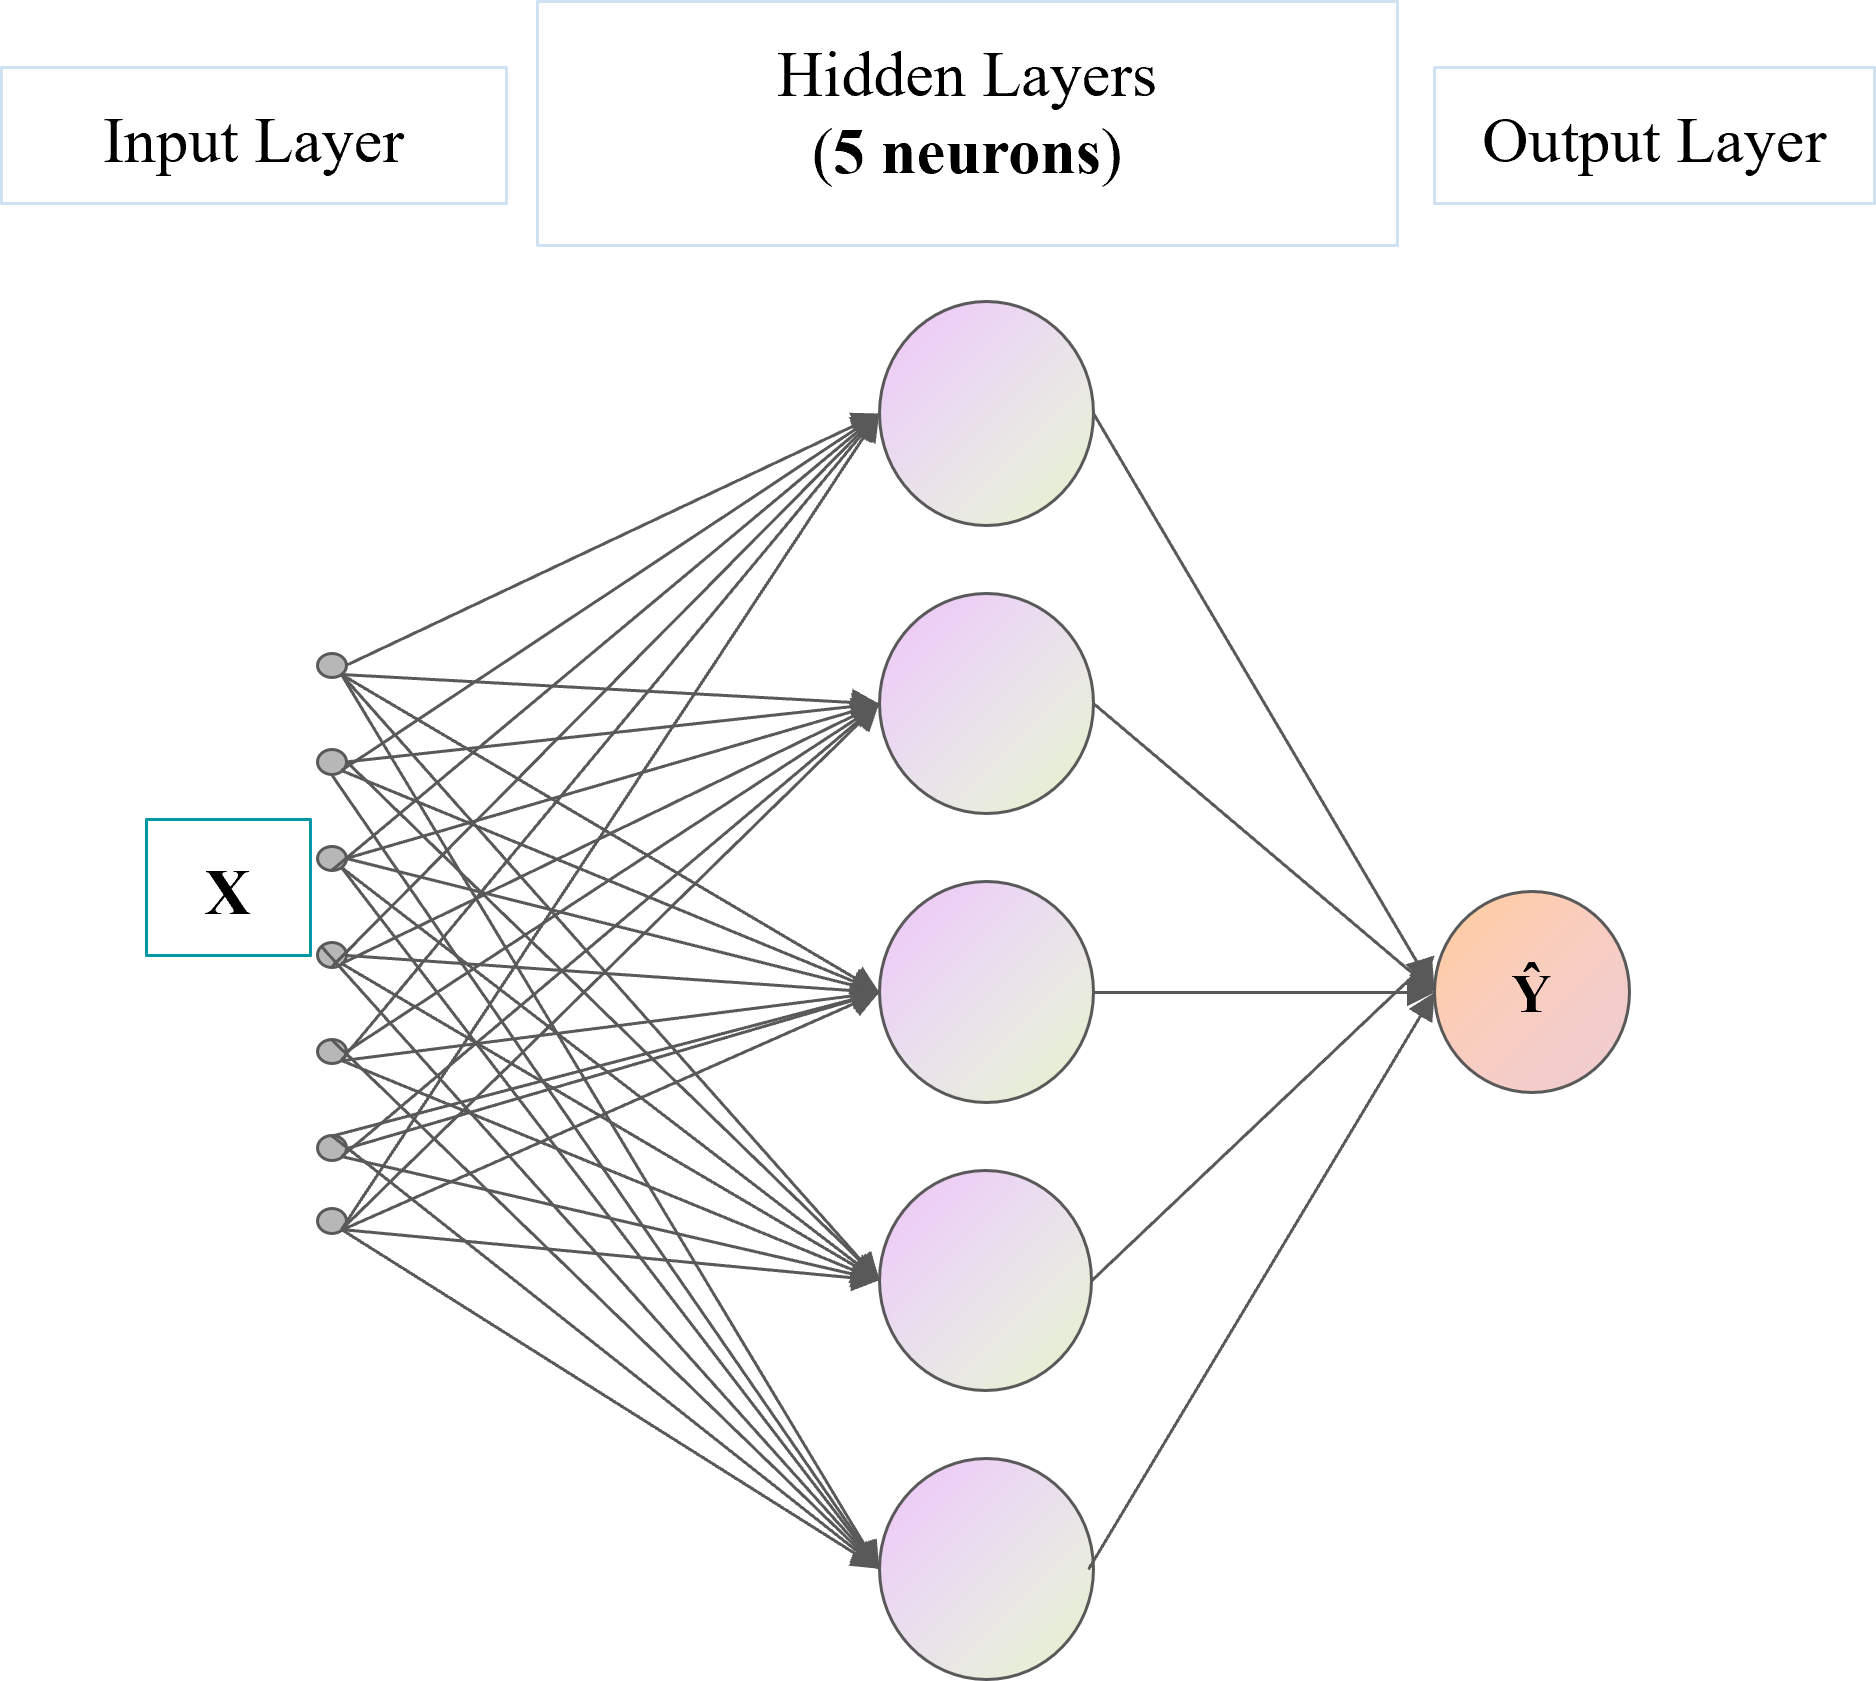
\includegraphics[width=\textwidth]{./figures/tropical_model.png}
		\caption{tropical model}
	\end{subfigure}
	\begin{subfigure}[b]{0.3\textwidth}
		\centering
		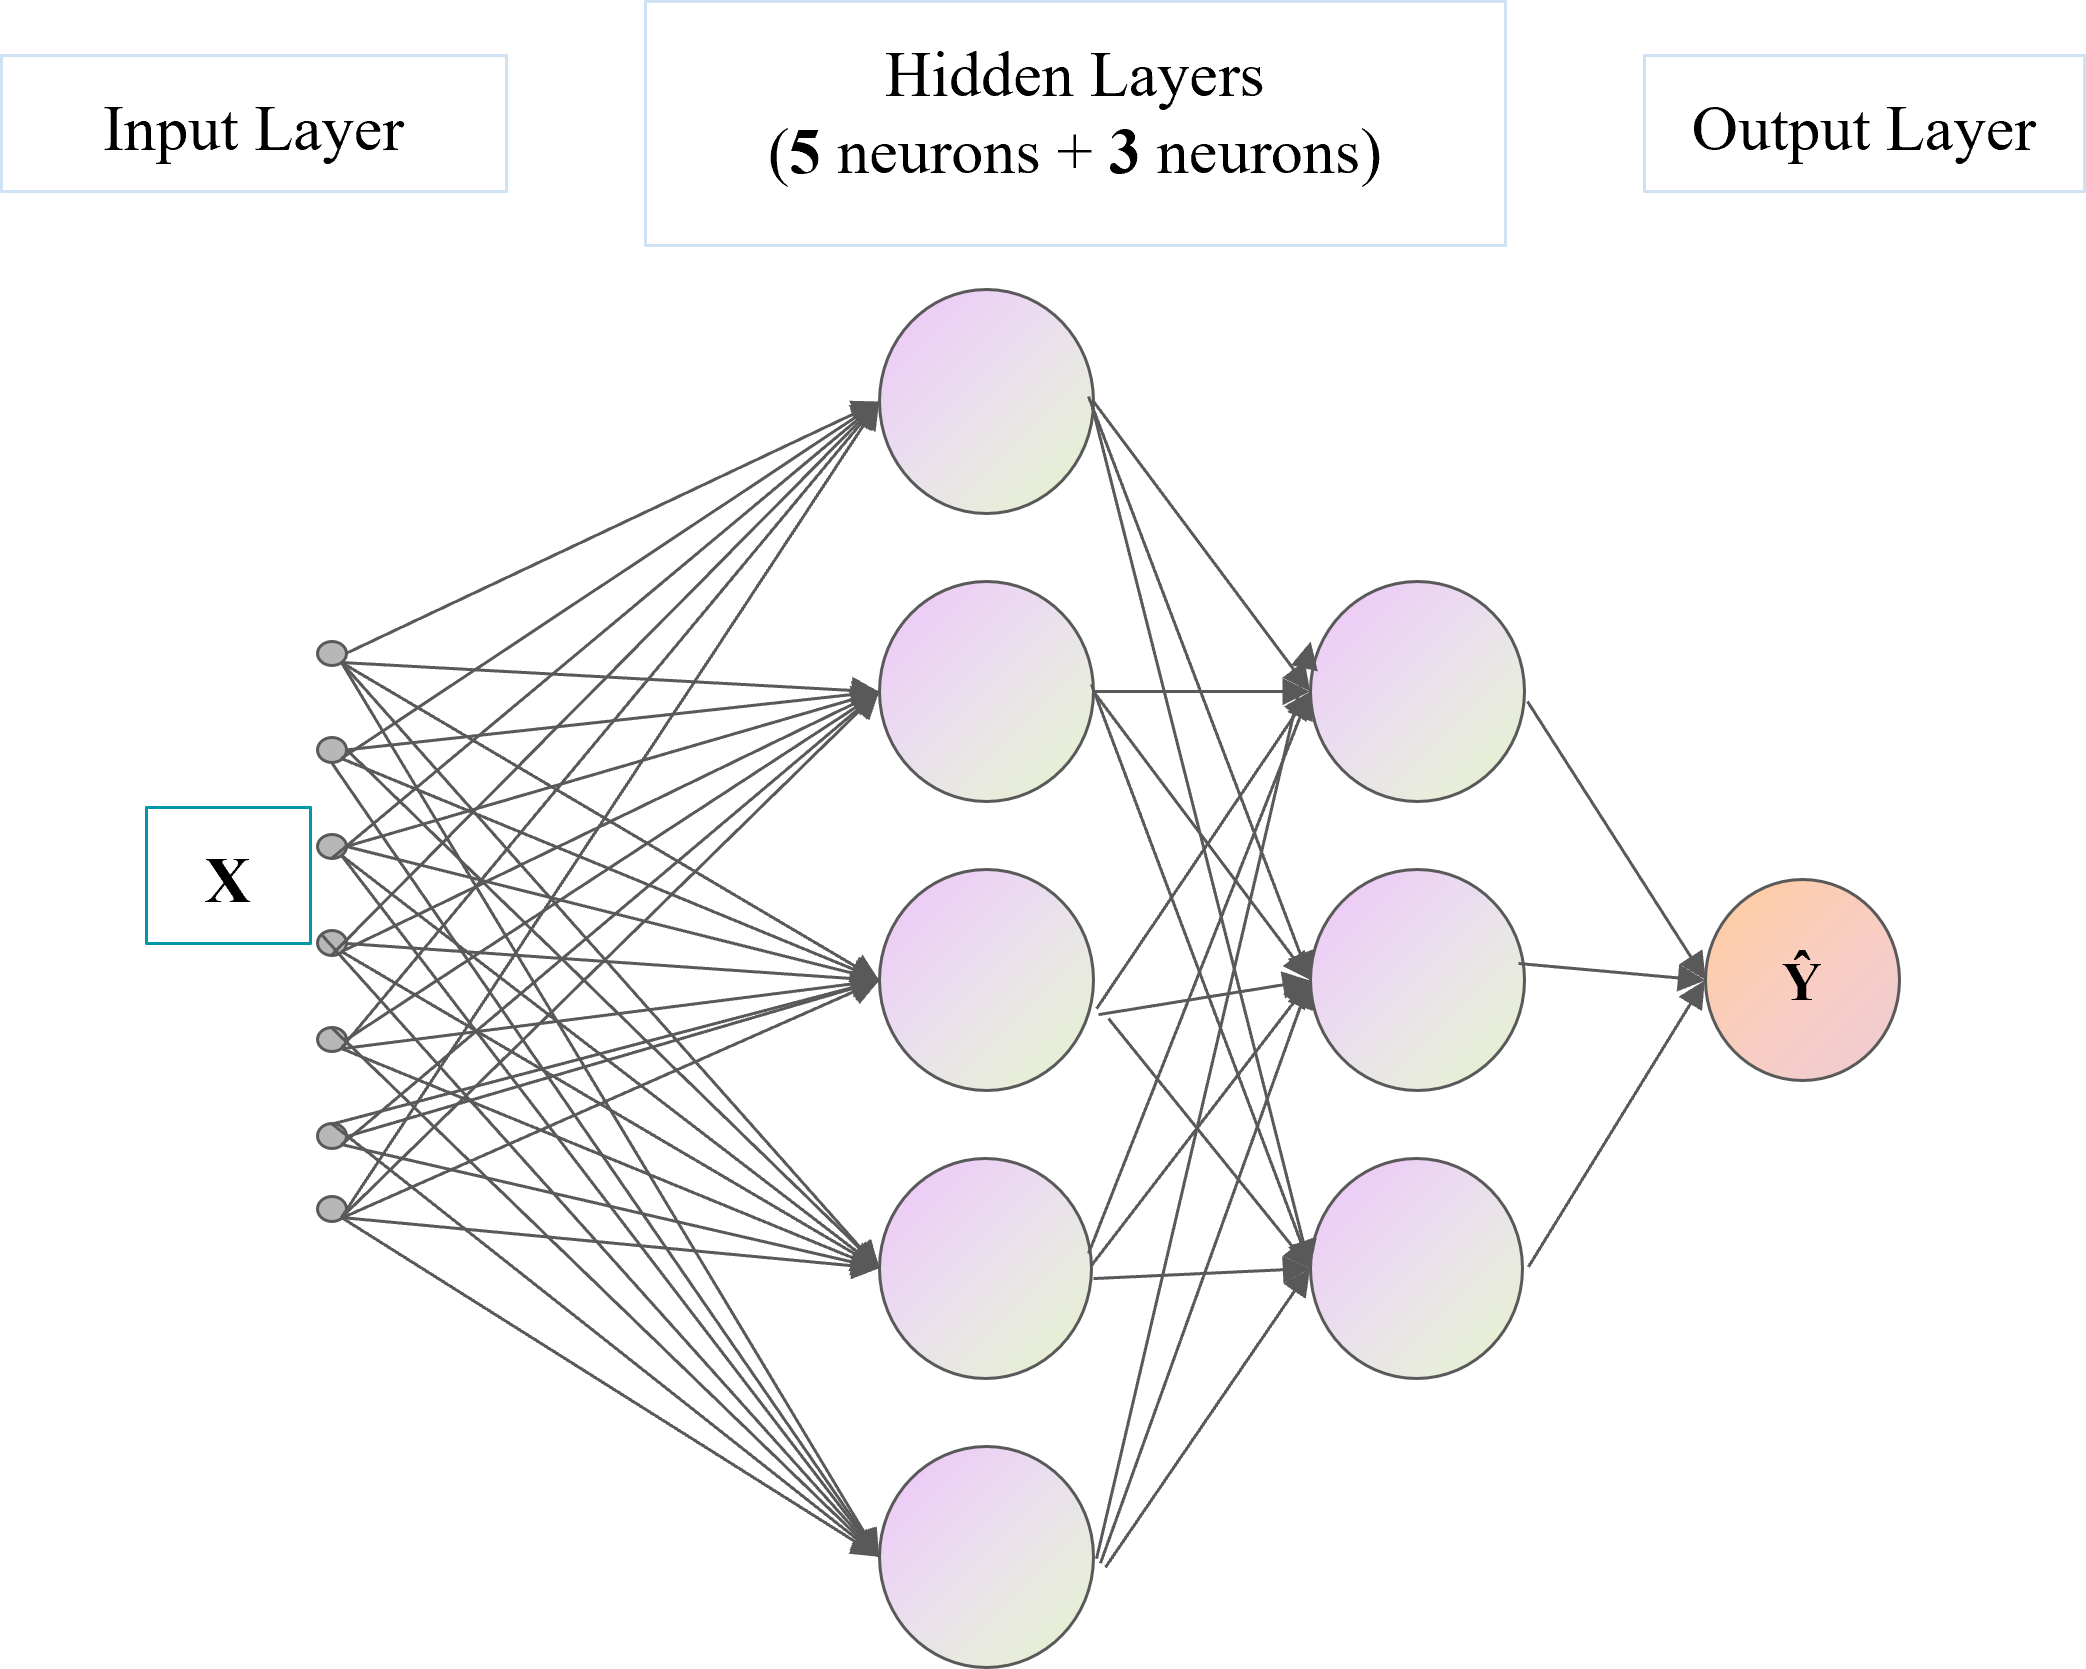
\includegraphics[width=\textwidth]{./figures/temperate_model.png}
		\caption{temperate model}
	\end{subfigure}
	\begin{subfigure}[b]{0.3\textwidth}
		\centering
		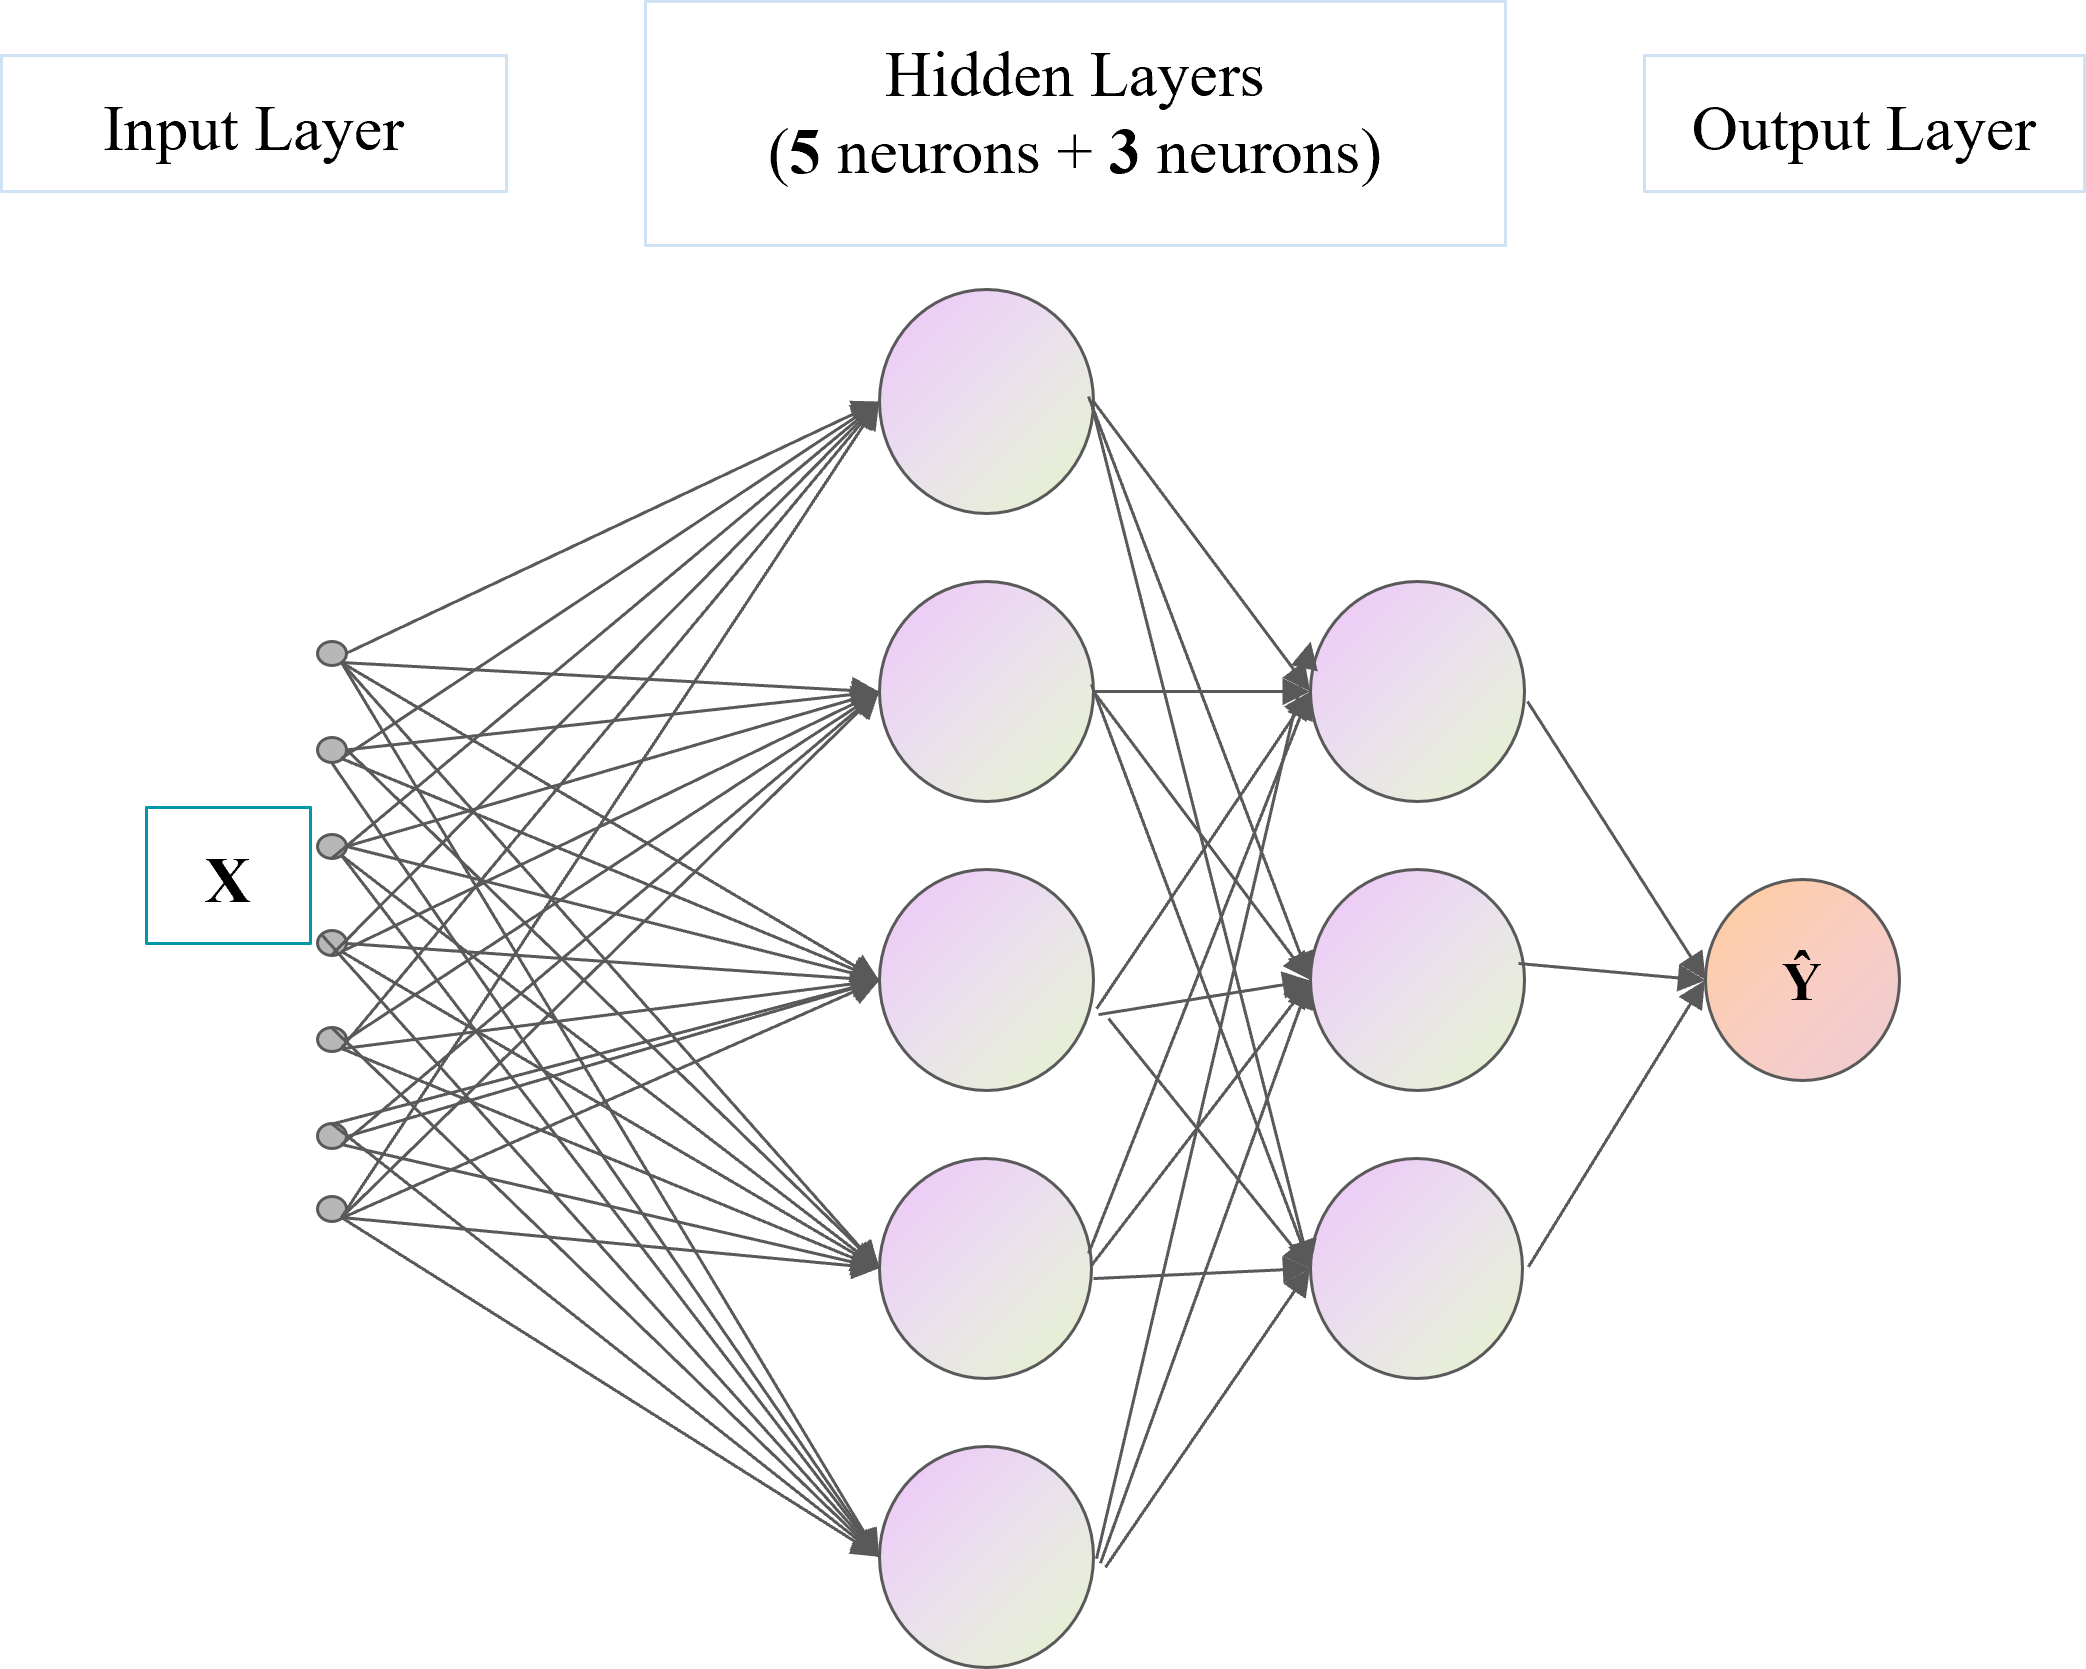
\includegraphics[width=\textwidth]{./figures/polar_model.png}
		\caption{polar model}
	\end{subfigure}
	\caption{\textbf{models built for training on diverse climate zones}}
	\label{models}
\end{figure}

Mean Square Loss(depicted in equation \ref{L2Loss()})was chosen as the loss function, with small gradient descent as the optimization algorithm for three models. Take the tropical model as an example, its calculation process can be described as$\textbf{Y} = \textbf{X}\cdot\textbf{W} + \textbf{b}$, where \textbf{Y}, \textbf{X},\textbf{W},\textbf{b} respectively stands for the label metric, feature metric, weights and bias, as is illustrated in formula \ref{metric}. 
\begin{equation}
	L(\textbf{w},b)=\frac{1}{\mathbb{B}}\sum_{i=1}^{\mathbb{B}}=\frac{1}{n}\sum_{i=1}^{\mathbb{B}}\frac{1}{2}(\textbf{w}^T\textbf{x}^{(i)}+b-y^{(i)})^2
	\label{L2Loss()}
\end{equation}
\begin{equation}
	\textbf{Y}=\begin{pmatrix}
		y \\
	\end{pmatrix}
	\quad
	\textbf{X}=\begin{pmatrix}
	x_{11} & \dots & x_{14} \\
	\vdots & \vdots & \vdots \\
	x_{n1} & \dots & x_{n4} \\
\end{pmatrix}
	\quad
		\textbf{W}=\begin{pmatrix}
		\omega_{11}\\
		\vdots \\
		\omega_{n1} \\
	\end{pmatrix}
		\quad
	\textbf{b}=\begin{pmatrix}
		b_{11}\\
		\vdots \\
		b_{n1} \\
	\end{pmatrix}
	\label{metric}
\end{equation}

It's also worth noting that the value of $\textbf{W}$ can directly reflect the importance of each indicator which the model has been attached to. For instance, after training the tropical model exhibits the weight matrix as $(0.8051, 0.1788, 0.0369, 0.1923)^{\top}$, where the corresponding variables are $(\text{AGB, UGB, DWC, SCS})^{\top}$. It can be concluded that the above-ground biomass(AGB) shoulders the most responsibility regarding the overall carbon sequestration of tropical forests, which also aligns with numerous existing researches that the under-tree plants are crucial to the stability of tropical ecosystems. Similar methods can be conducted on the analysis of temperate model and polar ones.

All the MLP networks form the generator of our CSGDN model. Hence, forest carbon sequestration values can be easily calculated by applying the generator to different regions. To validate the effectiveness of our model, we also build test datasets including datas of Canada, Brazil and China, which are collected from \cite{1}. All of the MLP models are fully tested and results are displayed in table \ref{us}. Due to the figures: $\text{model estimation}\approx\text{real value}$, it can be concluded that our model exhibits strong robustness as well a generalizability, which can be used to estimate the carbon sequestration of a specified region.

\begin{table}[h]
	\centering
	\setlength{\tabcolsep}{2pt}
	\begin{adjustwidth}{-0.135\textwidth}{}
	\begin{tabular}{cccccccc}
		\toprule[2pt]
		\textbf{variables} & \textbf{TGS}$(m^3/ha)$ & \textbf{AGB}$(t/ha)$ & \textbf{UGB}$(t/ha)$ & \textbf{DWC}$(t/ha)$ & \textbf{SCS}$(t/ha)$ & \textbf{model estimation}$(t/ha)$ & \textbf{real value}$(t/ha)$ \\
		\midrule[1pt]
		\textbf{Canada(1990)} & 136.747 & 95.09 & 23.47 & 41.35 & 82.21 & 212.72 & 210.01 \\
		\textbf{Canada(2010)} & 136.030 & 91.16 & 22.57 & 40.89 & 85.79 &211.55 & 211.82 \\
		\textbf{Canada(2016)} & 129.96 & 90.43 & 22.37 & 40.09 & 82.96 &206.72 & 207.88 \\
		\textbf{Canada(2020)} & 130.02 & 90.43 & 22.37 & 40.09 & 82.96 &206.76 & 207.88 \\
		\textbf{Brazil(2020)} & - & 171.92 & 40.79 & 10.43 & 41.37 &154.06 & 153.56 \\ 
		\textbf{Brazil(2016)} & - & 171.14 & 40.62 & 10.44 & 41.35 &153.40 & 152.99 \\
		\textbf{Brazil(1990)} & - & 163.60 & 39.07 & 10.42 & 41.82 &147.14 & 148.74 \\
		\textbf{Brazil(2010)} & - & 169.44 & 40.26 & 10.49 & 41.25 &151.95 & 151.96 \\
		\textbf{China(2010)} & 74.58 & 55.72 & 14.31 & 11.23 & 1.30 &39.56 & 38.65 \\
		\textbf{China(2016)} & 82.03 & 61.76 & 15.75 & 12.50 & 1.22 &43.63 & 43.75 \\
		\textbf{China(2018)} & 84.37 & 63.26 & 16.09 & 12.28 & 1.20 &44.78 & 44.56 \\
		\textbf{China(2020)} & 87.24 & 64.72 & 16.43 & 12.07 & 1.182 &46.08 & 45.72 \\
		\bottomrule[2pt]
	\end{tabular}
	\end{adjustwidth}
	\label{us}
	\caption{\textbf{validation of the generator-MLP model on real data.}}
\end{table}  

While giving an accurate estimation of $FCS$, the generator model also reveals the differences across climate zones as well as the $FCS$ shifting trend within a single climate zone, as is illustrated in Figure \ref{predicts}.


\begin{figure}[h]
	\centering
	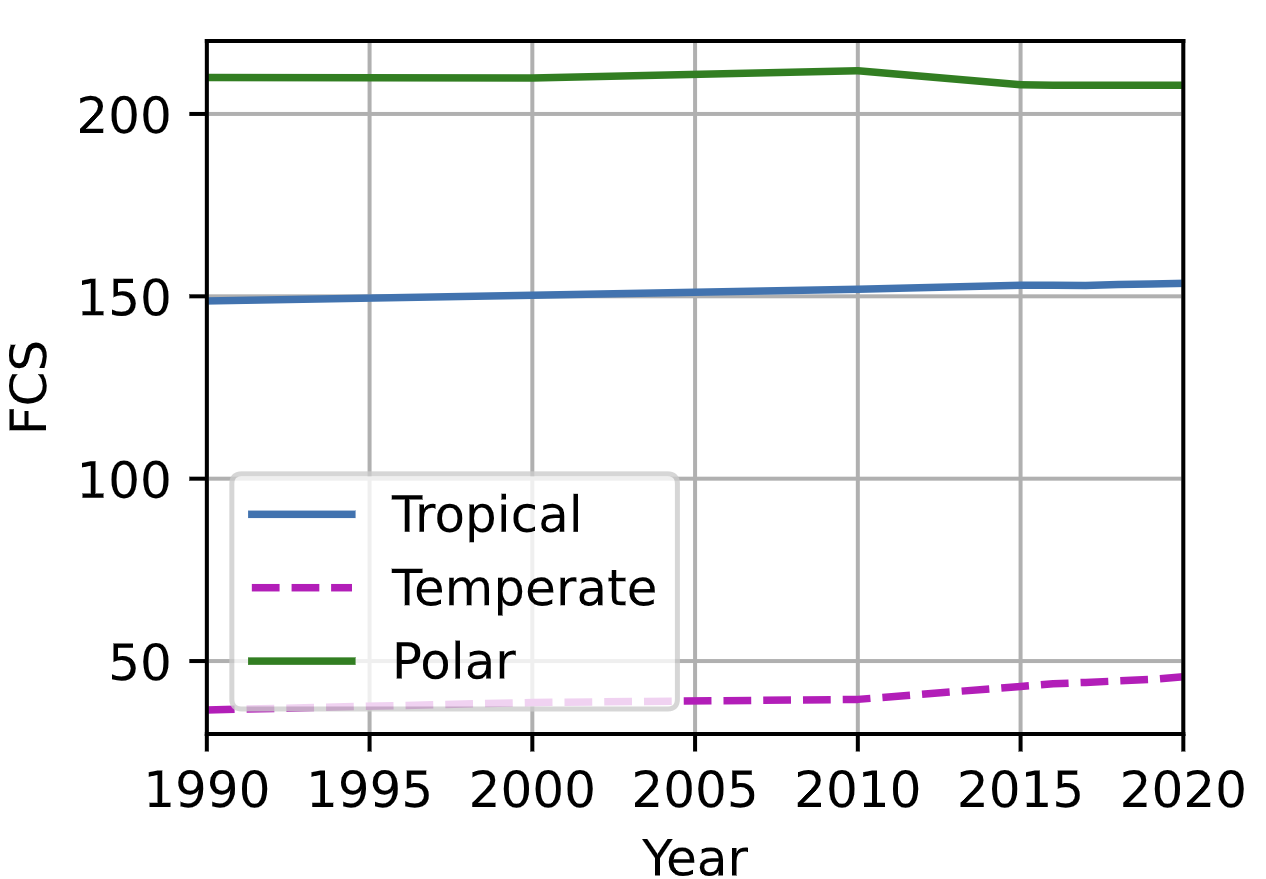
\includegraphics[width=0.5\textwidth]{./figures/comparis.png}
	\caption{\textbf{Visualization of model predictions.}}
	\label{predicts}
\end{figure}

Between different climate zones, it can be seen that $FCS_{\text{Polar}}>FCS_{\text{Tropical}}>FCS_{\text{Temperate}}$. Climate discrepancy is the major contributor of the result. In polar areas where temperatures stay at a freezing level, metabolism of forest plants deteriorate drastically. Meanwhile, the warm living conditions of tropical ecosystems lead to an increase in the consumption of carbon resources, making it harder for the forests to sequestrate carbon.


However, the generator model itself is insufficient to comprehensively describe the real carbon sequestration of a specified forest, since the model lays its foundation on an ideal premise that carbon sequestrated in plants will be stored in forests for eternity and ignored humans' impact on the sequestration process, such as the commercial utilization of timbers. Hence, we propose a deterioration model, called as carbon-deterioration model(CDM) to simulate people's exploit of forests and its influence introduced on carbon sinks. CDM functions similarly as the discriminator in GAN, but differs in its working principles.

\subsection{The discriminator-CDM model}
\subsubsection{Establishment of the global generator model}
\hspace{2em} Notice that carbon sequestration process is tightly bonded with time, we primarily measured the correlation between time and pivotal elements in the generator network(such as $TGS, AGB$) and mapped the neural network to time dimension, which could be depicted as equation \ref{transfer}, where $\textbf{T}(\cdot)=(\alpha(\cdot),\beta(\cdot),\theta(\cdot),\gamma(\cdot),\epsilon(\cdot))^{\top}$ 
\begin{equation}
	FCS = \textbf{Indicators}\cdot\textbf{W}\hspace{1em} 
	\text{where}\hspace{1em}\textbf{Indicators} = 
	{\begin{pmatrix}
		TGS \\ AGB \\ UGB \\ DWC \\ SCS
	\end{pmatrix}}^{\top}=\textbf{T}(t), 
	W=\begin{pmatrix}
		\sigma_1 \\ \sigma_2 \\ \sigma_3 \\ \sigma_4 \\ \sigma_5 
	\end{pmatrix}.
	\label{transfer}
\end{equation}

Then we employed \textbf{MATLAB} to determine the specific form of $\textbf{T}(\cdot)$, which is illustrated in table \ref{nihe}.
\begin{table}[h]
	\centering
	\setlength{\tabcolsep}{25pt}
	\begin{adjustwidth}{-0.06\textwidth}{}
	\begin{tabular}{cccccc}
		\toprule[2pt]
		region & $\sigma_1$ & $\sigma_2$ & $\sigma_3$ & $\sigma_4$ & $\sigma_5$ \\
		\midrule[1pt]
		tropical forests & - & 0.805 & 0.179 & 0.037 & 0.192 \\
		temperate forests & 0.327 & 0.241 & 0.071 & 0.066 & 0.008 \\
		polar forests & 0.789 & 0.543 & 0.144 & 0.259 & 0.500 \\
		\bottomrule[2pt]
	\end{tabular}
	\end{adjustwidth}
	\caption{\textbf{Weights of generator model after being mapped to time dimension.}}
\end{table}

\begin{table}[h]
	\centering
	\begin{tabular}{cccc}
		\toprule[2pt]
		elements & tropical model & temperate model & polar model \\
		\midrule[1pt]
		$\alpha(t)$ & - & $0.6996\times t-1327.845$ &  $-0.2632\times t+661.1045$ \\
		$\beta(t)$ & $0.283\times t -399.64$ & $0.4394 \times t -824.0494$ & $-0.182\times t + 457.7236$ \\
		$\theta(t)$ &$3.3042\times t -6565.7953$ & $0.0979\times t -181.6473$ &$-0.0427\times t + 108.4636$ \\ 
		$\gamma(t)$ &$-0.0003\times t + 10.9878$ &$0.079\times t -147.1069$ & $-0.0319\times t + 104.5928$\\
		$\epsilon(t)$ &$-0.0162\times t + 73.9372$ &$-0.0157\times t + 32.9147$ &$0.0203\times t+42.3389$\\
		\bottomrule[2pt]
	\end{tabular}
	\label{nihe}
	\caption{\textbf{the specific form of $\textbf{T}(\cdot)$}}
\end{table}
Hence, the time-based form of generator model goes as:
\begin{equation}
	\begin{cases}
		FCS_{tropical}=0.816\times t - 1482.385 \\
		FCS_{temperate} = 0.347\times t - 655.14 \\
		FCS_{polar} = -0.31\times t + 834.033
	\end{cases}
	\label{time}
\end{equation}

Additionally, we calculate the global model of forest carbon sequestration, which goes as:
\begin{equation}
	FCS_{global} = \mu_1\times FCS_{tropical} + \mu_2 \times FCS_{temperate} + \mu_3 \times FCS_{polar}
\end{equation}

Where $$\mu_1 = \frac{S_{tropical}}{S_{earth}}\approx0.4,  \mu_2 = \frac{S_{temperate}}{S_{earth}}\approx0.4,\mu_3 = \frac{S_{polar}}{S_{earth}}\approx0.2$$

Therefore, we have the global generator model which could predict the worldwide forest carbon sequestration regarding time as its variable $$FCS_{global}(\text{tons/ha}) = 0.4032\times t(\text{year}) -688.2034$$

\subsubsection{Establishment of carbon deterioration model(CDM)}
\hspace{2em} Based on the fact that generator model merely describes the sequestration process and ignored humans' consumption and interruptions, we build the CDM to present humans' impacts on forests.

Contemporary commercial industry mainly exploits the forests for economic purpose. Timbers are cut to produce goods such as tissues and furniture. These products can be categorized based on their lifespan, short-lifespan and long-lifespan respectively. Therefore, we use symbolic commodities of either group to quantificationally evaluate humans' impact on forest carbon sinks, which are paper and furniture respectively.

Datas have been reported that $tree\times1 = A4\times 3000$. We use the generator model to estimate the carbon storage of single tree and infer that $tree\times 1=carbon_{sequestration}\times20 \text{kg} $. Therefore, $A4\times 1 =carbon\times \frac{1}{150} \text{kg}$. Considering that humans' consumption on paper$\approx 4.1\times10^8 \text{tons}$ and $A4=5\text{g}$, we have the global carbon consumption on paper$\approx 0.0462$ tons per hectare annually. Similar
estimations can be conducted on the furniture industry.

However, since paper feature a much shorter lifespan than that of the furniture, in an annually evaluation the paper carbon consumption can be viewed as a constant. Furnitures, however, don't exhibit similar characteristic due to their long lifespan. Hence, considering the carbon which permanently stored in furnitures, we use arithmetic progression sequence to build the CDM model, which goes as :
\begin{equation}
	DCS_{global}\text{(tons·year/ha)} = 0.0462 - \sum_{i}^{t}x_i 
\end{equation}
where $x_i$ stands for the annual carbon sequestration of wooden furnitures and $t$ stands for the year evaluation being conducted. 
\section{Forest management plan under CSGDN model}
\subsection{Under the generator model}
思路就是，用神经网络的权重看哪个指标最重要然后分析哪个指标
\subsection{Under the CDM model}
\hspace{2em} First we define $FCS_{global} = F(\cdot), DCS_{global} = D(\cdot)$. 
思路就是，列出俩抽象函数，一个大于另一个的时候，该怎么样，一个小于另一个的时候该怎么样，相等的时候达到平衡
















%%%%%%%%%%%%%%%%%%%%%%%%%%%%%%
\newpage
\begin{thebibliography}{00}
\bibitem{1}
Fu Yujie, Tian Di, Hou Zhengyang, Wang Minggang, Zhang Naili. Review on the evaluation of global forest carbon sink function[J]. Journal of Beijing Forestry University, 2022, 44(10): 1-10.
\bibitem{2}%草稿
Oxford Advanced Dictionary pp.304--306 
\bibitem{3}
https://www.fao.org/forest-resources-assessment/fra-2020/country-reports/en/
\end{thebibliography}

\end{document}
\end
